\documentclass[10pt,twocolumn,letterpaper]{article}

\usepackage{cvpr}
\usepackage{times}
\usepackage{epsfig}
\usepackage{graphicx}
\usepackage{amsmath}
\usepackage{amssymb}

% Include other packages here, before hyperref.

% If you comment hyperref and then uncomment it, you should delete
% egpaper.aux before re-running latex.  (Or just hit 'q' on the first latex
% run, let it finish, and you should be clear).
\usepackage[breaklinks=true,bookmarks=false]{hyperref}

\cvprfinalcopy % *** Uncomment this line for the final submission

\def\cvprPaperID{****} % *** Enter the CVPR Paper ID here
\def\httilde{\mbox{\tt\raisebox{-.5ex}{\symbol{126}}}}

% Pages are numbered in submission mode, and unnumbered in camera-ready
%\ifcvprfinal\pagestyle{empty}\fi
\begin{document}

%%%%%%%%% TITLE
\title{A Transfer Learning Approach to DICOM Slice Selection}

\author{Kennan LeJeune\\
   % For a paper whose authors are all at the same institution,
   % omit the following lines up until the closing ``}''.
   % Additional authors and addresses can be added with ``\and'',
   % just like the second author.
   % To save space, use either the email address or home page, not both
   \and
   David Blincoe\\
   \and
   Sam Jenkins\\
   \and
   Chris Toomey\\
   \and
   Arthur Xin\\
   \and
   \\
   {Case Western Reserve University, Cleveland, OH}\\
   {\textit{Department of Computer and Data Sciences}}\\
   {\tt\small \{kennan, drb133, soj3, ctt16, sxx132\}@case.edu}
}
\maketitle
%\thispagestyle{empty}

%%%%%%%%% ABSTRACT
\begin{abstract}
   Lung tumor identification and classification is a challenging task which typically requires a trained medical
   professional to choose the best slices of a scan and accurately classify the chosen slices. With medical data privacy restrictions
   and regulations, it is difficult to collect sufficient data to construct a typical Convolutional Neural Network to
   choose and classify DICOM slices. We propose an inductive transfer learning approach which applies hidden layer
   image representations from a residual neural network to our lung nodule classifier to classify groups of slices and provide
   recommendations to a user as to what groups may contain possible benign or malignant nodules.
\end{abstract}

\section{Introduction} \label{sec:intro}

   Traditionally, Machine Learning problems rely on the assumption that the training data and future data domains
   are in the same feature space and have the same distribution (Pan, Yang). However, a large number of real world
   applications perform poorly when these assumptions are not met. A common instance of this is a classification task on
   a restricted domain of interest (e.g. classifying malignant brain tumors) with minimal or unlabeled training data,
   but we have sufficient training data in another domain of interest (e.g. classifying malignant lung carcinomas).
   Transfer Learning aims to solve this problem by adapting the knowledge acquired from a training task or
   training domain for use in a related domain or task. Intuitively, we can apply a solution to a problem to a
   different but related problem in a human-like matter.

   \subsection{Formal Transfer Learning Definition} \label{sec:intro-def}
      Given source and target domains $D_S, D_T$ and learning tasks $T_S$ on the source domain and $T_T$ on the target
      domain, where we aim to improve the learning of a target predictive function $f_T(\cdot)\in D_T$ using
      the knowledge in $D_S$ or $T_S$, where $D_S\neq D_T$ or $T_S\neq T_T$. Note that in the case where both domains
      and tasks are equivalent, this is analogous to a standard machine learning problem. We can characterize the
      nature of nearly all Transfer Learning problems by considering three primary cases:

   \subsection{Types of Transfer Learning} \label{sec:intro-types}

      1. $D_S = D_T, T_S\neq T_T$ (Inductive Transfer, \ref{sec:intro-types-inductive})
    
      2. $D_S\neq D_T, T_S = T_T$ (Transductive Transfer, \ref{sec:intro-types-transductive})
    
      3. $T_S\neq T_T$ and $D_S, D_T$ are unlabeled (Unsupervised Transfer, \ref{sec:intro-types-unsupervised})
    
      \subsubsection{Inductive Transfer Learning} \label{sec:intro-types-inductive}
    
         In Inductive Transfer Learning, the domain of the source and target tasks is the same. In this case, labeled data
         from the target task must be available in order to induce the predictive function that we want the classifier to learn.
         There are two situations in inductive transfer learning: one where labeled source data is available, and one where it
         is not. The first scenario is similar to something known as self-taught learning, in which the classifier hopes to
         learn basic patterns from random unlabeled data. The second scenario is similar to multi task learning, where the
         classifier attempts to learn several classification tasks at the same time, except in this case we only care about
         the performance on a single target task, and are hoping to use knowledge learned from the other tasks in order to
         improve performance on said target task.
    
      \subsubsection{Transductive Transfer Learning} \label{sec:intro-types-transductive}
         Transductive Transfer Learning focuses on an area in which the source and target tasks are the same, but the domains
         differ. The data used in the target domain is unlabeled, whereas there is an abundance of labeled data in the source
         domain. Transductive transfer learning can be broken down even further, into two specific scenarios: the first, in
         which the target and source domains have a different feature space; and the second, where the feature space is the
         same, but the input data have different marginal probability distributions.
    
      \subsubsection{Unsupervised Transfer Learning} \label{sec:intro-types-unsupervised}
         Unsupervised Transfer Learning focuses on a setting where there is no labeled data for either the source and target
         domains, and the target task is different from the source task. This situation is common in areas such as clustering
         and dimensionality reduction.

\subsection{Classification Problem} \label{sec:intro-class}
	Lung cancer is one of the most lethal diseases worldwide. A patient’s probability of survival decreases the longer it takes to identify a cancerous tumor. Thus, successful lung cancer screenings can be used to save countless lives, making them extremely valuable. Manually inspecting cancer screenings can be very time and cost intensive, and is not necessarily error free, as classifying tumors requires advanced radiological knowledge. Computer programs, and deep learning specifically, can therefore help enhance the quality and decrease the costs associated with analyzing screenings. Given the scarcity of tumors in cancer screenings, however, and their limited availability in general, it is difficult to train models. Therefore, we can use transfer learning to learn the feature representation of images and transfer that knowledge to cancer screenings, so it does not have to learn the representation itself and can focus specifically on classifying benign or malignant tumors.

%-------------------------------------------------------------------------

\section{Related Works} \label{sec:related}

   \subsection{Machine Learning vs Deep Learning Algorithms} \label{sec:related-dl-vs-ml}
      In the paper by \cite{ml_vs_dl}, the authors sought out to systematically compare the results and algorithms of
      several works of literature regarding the detection of lung modules in the LIDC-IDRI database.
      Out of the initial 1972 publications found in their search, the authors assessed the eligibility of 180 papers
      and found only 41 of which satisfied their for data requirements and were thus considered for their discussion.

      Amongst the algorithms found in the feature-based framework in the machine learning category, the most popular
      type was the Support-vector Machines (SVM). The algorithms that implemented some forms of the SVM classifier
      reached accuracy range of 68.4\%-99.0\%, sensitivity range of 55.0\%-98.6\%, specificity range of 87.5\%-98.2\%, and
      and AUC of 0.905-0.998.
    
      Amongst the algorithms that were used in the deep learning category, the convolution neural network (CNN) was the most
      frequently used type. The algorithms that implemented a CNN architecture had an accuracy range of 82.2\%-97.6\%,
      sensitivity range of 83.1\%-96.6\%, specificity range of 71.4\%-98.2\%, and an AUC range of 0.877-0.984.

   \subsection{Deep Residual Networks} \label{sec:related-deep-residual-networks}


   \subsection{Nodule Malignancy Classification} \label{sec:related-nodulex}


\section{Datasets} \label{sec:data}
   For standard transfer learning, both source and target data is needed. In this case
   the project utilizes ResNet 50's weights of the source images. The data that the weights
   were trained on comprises source domain, $D_s$.

   LIDC-IDRI, \ref{sec:data-lidc}, is used to train the output segment of the
   the network. This is our target domain, $D_t$.

   \subsection{LIDC-IDRI Dataset} \label{sec:data-lidc}
      The Lung Image Database Consortium image collection (LIDC-IDRI) dataset
      is a very popular cancer classification dataset that focuses on tumors located
      in the lungs. The lung scans are CT images of the upper torso. The entire dataset
      consists of 1018 cases that each contain thoracic radiologists annotations of tumor segments
      These tumors annotations each contain 9 different descriptors such as malignancy,
      calcification, and lobulation. The descriptor this paper is interested in is the
      malignancy of each nodule.

      The malignancy is rated on a 1-5 scale. 1 being 'Highly Unlikely' of malignancy and
      5 being 'Highly Suspicious' of malignancy. Using these ratings each slice in a chest CT
      was rated as either malignant, benign, or non-nodule. A slice was considered non-nodule
      if there was no nodule annotations found within the slice. To split nodules into malignant
      and benign labels, the annotations performed on a specific node were averaged and for malignancy
      values $\ge 3$, the node was considered malignant and for malignancy values $< 3$, the node was
      considered benign, based upon the 4 radiologists predictions.
    
      \subsubsection{PyLIDC} \label{sec:data-lidc-pylidc}
         To assist in the extraction of data from the DICOM image files, a python library was utilized
         to read to XML files which contained the annotation information for each nodule. \cite{Hancock2018}
    
      \subsubsection{Processing LIDC-IDRI Data} \label{sec:data-lidc-processing}
         DICOM files, (Digital Imaging and Communications in Medicine), are the standard method for transferring
         and communicating image data. The structures of these files are extremely robust and offer many access in
         the form of 'Tags'. In the case of LIDC-IDRI, the dataset is composed entirely of CT images which must be
         processed by first transforming the image data along the HU (Hounsfield scale) given the transformation
         coefficients in the DICOM.
    
         The vertical slice size must also be taken into account because CT scans can be ordered in a variety of
         ranging resolutions from $(<0.1\text{mm to } >3 \text{mm})$. A scale of 1 mm per slice was chosen and the
         pixel data was transformed.

\section{Project Structure} \label{sec:struct}

   \subsection{Residual Neural Network} \label{sec:struct-cnn}
        The vanishing gradient has long been a problem when constructing neural networks with large architectures. Essentially, the back-propagating the gradient to earlier layers makes the gradient tend towards zero, so the performance can degrade in earlier layers. This can result in worse performance for deeper models than shallower ones, since earlier layers will perform worse for the deeper model. Residual neural networks attempt to solve this problem, by using "shortcuts" that jump layers in order to make sure the gradient does not become infinitesimally smaller. Figure \ref{fig:struct-cnn-residual} illustrates this concept. The input, $X$, is both passed to the next layer and skips ahead to the layer after, in order to add the effects of the input and the activation function and avoid the vanishing gradient problem.

        \begin{figure}[h]
            \centering
            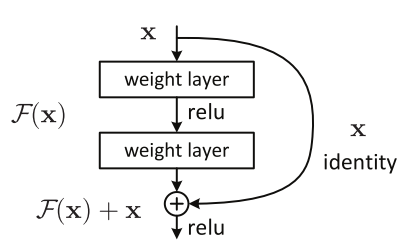
\includegraphics[width=0.4\textwidth]{./images/residual.png}
            \caption{Residual Node}
            \label{fig:struct-cnn-residual}
        \end{figure}
    
        For our project, we are using the ResNet-50, \ref{fig:struct-cnn-resnet},pre-trained model for Keras. The architecture of the model can be seen in the image below.
    
        \begin{figure*}
            \begin{center}
                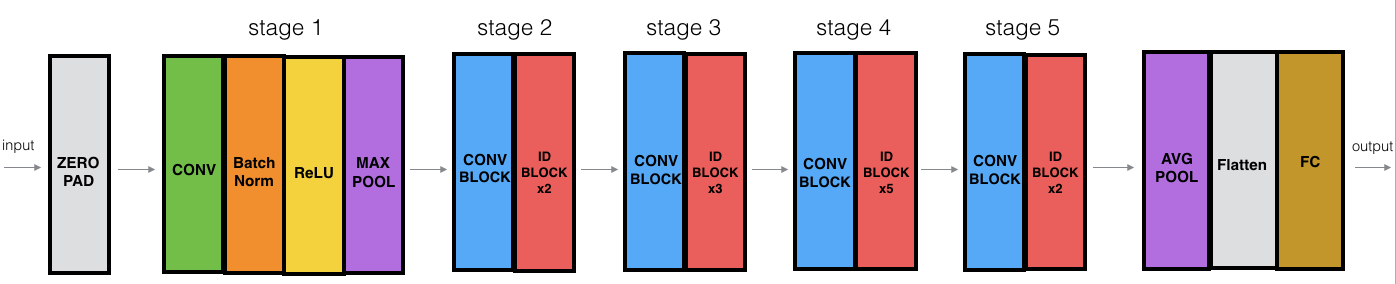
\includegraphics[width=\textwidth]{./images/Resnet-50.png}
            \end{center}
            \caption{Architecture of ResNet-5}
            \label{fig:struct-cnn-resnet}
        \end{figure*}
    
         As a whole, the model has 5 stages, followed by a pooling and flattening step to output the data. The first stage puts the data through a convolutional layer that then runs ReLU and max pooling, and then the model consists of four stages convolutional blocks and identity blocks, with varying number of identity blocks. The convolutional blocks runs the input through two iterations of convolutional layers, followed by ReLU, and a final convolutional layer, and adding to this the input run through a convolutional layer, before running a final iteration of ReLU. The identity block does the same, but simply adds back the input in the end rather than a convolutional layer run on the input. The difference in the two is the shape of the input and output: if their dimensions line up, then an identity block is sufficient, otherwise the input must be re-shaped to match the output.

   \subsection{Model Sectors} \label{sec:struct-sector}

        A unique approach of our solution is to bin together specific locations of lung CT scans. In other words, there exists
        a hyper-parameter called {\it sector\_num}$=x$ that will train $x$ independent ResNet models, \ref{sec:struct-cnn} on separate
        physical portions of the CT scans. For example, every studies full chest CT scan was scaled to be just 65 slices. If the {\it sector\_number} $=13$,
        there will be 13 bins starting with bin 1 at the top of the chest and bin 13 at the bottom. Here, each bin will be comprised
        of $5$ slices from each study.
    
        Once there are $x$ independent CNN models trained, the output of the classifier given a study will
        be the slice numbers that should be looked at closely.

\section{Experiments} \label{sec:experiments}
   Three primary ideas were tested in this project. One was to determine if this model generally performed well on the given data and if it performed well
    compared to the results from \ref{sec:related-dl-vs-ml}. The second goal was to analyze if shifting the 
   {\it sector\_num} as seen in \ref{sec:struct-sector}, increased or decreased the performance of our model. The third was to see if down-sampling the 
   given CT scans to a lower resolution contributed to a significant drop in accuracy.

   \subsection{General Performance} \label{sec:experiments-general-performance}
        Sectors #13, Image 224x224
   \subsection{Varying Sector Number} \label{sec:experiments-sector}

   \subsection{Varying Image Resolution} \label{sec:experiements-res}

\section{Results} \label{sec:results}

\section{Further Investigation} \label{sec:further}

​	There are two general problems within the broader classification problem: first, identifying whether a lung has a tumor and, if it does, classifying that tumor as malignant or benign. Further work can be broken down into these two subsections

​	\subsection{Identifying Tumors} \label{sec:id-tumor}

​		One approach to tumor identification is the use of autoencoders rather than CNNs or residual neural networks. In the autoencoder context, \ref{sec:related-dl-vs-ml} gives some context on how autoencoders have been used in this area. In one such example, lung cancer screenings with tumors are input into the autoencoder, and initially, the output is the same size as the input and identifies the tumor, with the rest of the picture blank (i.e. it only identifies the tumor in the output). This process is repeated and the autoencoder learns how to identify the varying shapes and sizes of tumors within lungs. This extension could be paired with another algorithm, like ours, to identify whether a tumor is malignant or benign. 

​	\subsection{Classifying Tumors} \label{sec:classify-tumor}

​		Once we can identify a tumor in a lung, the problem becomes whether that tumor can be harmful. \ref{sec:related-deep-residual-networks} uses ResNet in a slightly different way than our implementation. Rather than scanning a full lung, they use an image of the tumor itself instead, and with this image, they create three images from this original image, each representing the different axes of the image (coronal, sagittal, and axial). Each of these is then input into a corresponding ResNet, setting up three different models. In order to both identify and diagnose a tumor, we could use a similar method to that used in \ref{sec:related-deep-residual-networks}. First, in order to identify the tumor, we could run along the coronal plane of a scan. Then, when we have identified the slices of the lung that have a tumor (if it exists), we can use all three planes (coronal, sagital, and axial) in order to diagnose the tumor. This would allow us a full dimension worth of data more than we are currently using, so it likely would help with accuracy. 

\section{Conclusion} \label{sec:conclusion}



{\small
\bibliographystyle{ieee}

\bibliography{egbib}
}

\end{document}
